\documentclass[conference]{IEEEtran}
\IEEEoverridecommandlockouts
% The preceding line is only needed to identify funding in the first footnote. If that is unneeded, please comment it out.
\usepackage{cite}
\usepackage{amsmath,amssymb,amsfonts}
\usepackage{graphicx}
\usepackage{textcomp}
\usepackage{xcolor}
\def\BibTeX{{\rm B\kern-.05em{\sc i\kern-.025em b}\kern-.08em
    T\kern-.1667em\lower.7ex\hbox{E}\kern-.125emX}}
\title{
\vspace{1cm}
{
\includegraphics[width=0.15\textwidth]{iithlogo.jpg} \\ Platformio Assignment} }
\author{Patnam Keerthi \\ Roll No: FWC22306 \\ patnamkeerthi4545@gmail.com}
 \begin{document}
\maketitle

 \section {ABSTRACT}
This document analyzes an asynchronous counter built with two JK flip-flops. The counter's sequence and the impact of the asynchronous design are examined.

What are the counting states (Q1,Q2) for the counter shown in the figure 1

 \begin {figure}[h]
 \centering
 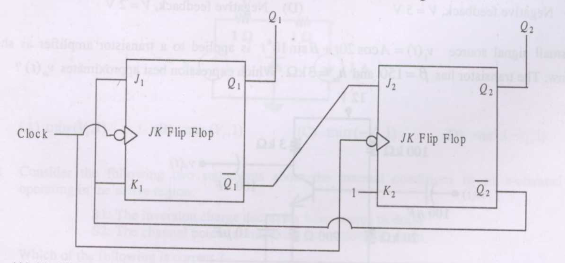
\includegraphics[width=0.35\textwidth]{seq.jpg}
 \caption{\label{fig: Sequential Circuit}}
 \end {figure}

 \section{COMPONENTS}
 \begin{table} [htbp]
\centering
\begin{tabular}{| c | c | c |} \hline
Components & Value & Quantity \\\hline
LEDs &  & 2 \\ \hline
Arduino & UNO & 1 \\ \hline
Jumper Wires &  & 10 \\ \hline
Breadboard & & 1 \\ 
\hline
\end{tabular}
\vspace{0.1cm}
\caption{\label{tab:widgets}}
\end{table}

\section{PROCEDURE}
\begin{itemize}
    \item \textbf{Power Supply:} Connect the Arduino board to a 5V power supply.
    \item \textbf{Clock Input:} Connect one end of a push button to digital pin 2 (clockPin) and the other end to +5V.
    \item \textbf{Q1 Output:} Connect the anode (longer leg) of an LED to digital pin 12 (Q1). Connect the cathode (shorter leg) of the LED to a 220-ohm resistor, and then to ground.
    \item \textbf{Q2 Output:} Connect the anode of another LED to digital pin 13 (Q2). Connect the cathode to a 220-ohm resistor, and then to ground.
\end{itemize}

 \section{RESULT}
 The Arduino code successfully implements a JK flip-flop using software. The circuit generates a specific sequence of outputs based on the clock input.


 Download the code given in the link below and execute them to see the output as shown in Fig.2  \\
https://github.com/patnamkeerthi4545/Fwc/blob/main/Platformio/main.cpp


\begin{table}[ht]
\centering
\label{tab:connections}
\begin{tabular}{|c|c|c|c|c|c|c|c|c|}
\hline
\multicolumn{2}{|c|}{Present state} & \multicolumn{4}{c|}{Present input} & \multicolumn{2}{c|}{Next state} \\ \hline
	Q1 & Q2 & J1 & K1 & J2 & K2 & $Q1^{+}$ & $Q2^{+}$ \\ \hline
	0 & 0 & 1 & 1 & 1 & 1  & 1 & 1 \\ \hline
	1 & 1 & 0 & 0 & 0 & 1 &  1 & 0 \\ \hline
	1 & 0 & 1 & 1 & 0 & 1 & 0 & 0 \\ \hline
	0 & 0 & 1 & 1 & 1 & 1 & 1 & 1 \\ \hline
\end{tabular}
\end{table}

 \begin{figure}[h]
   \centering
   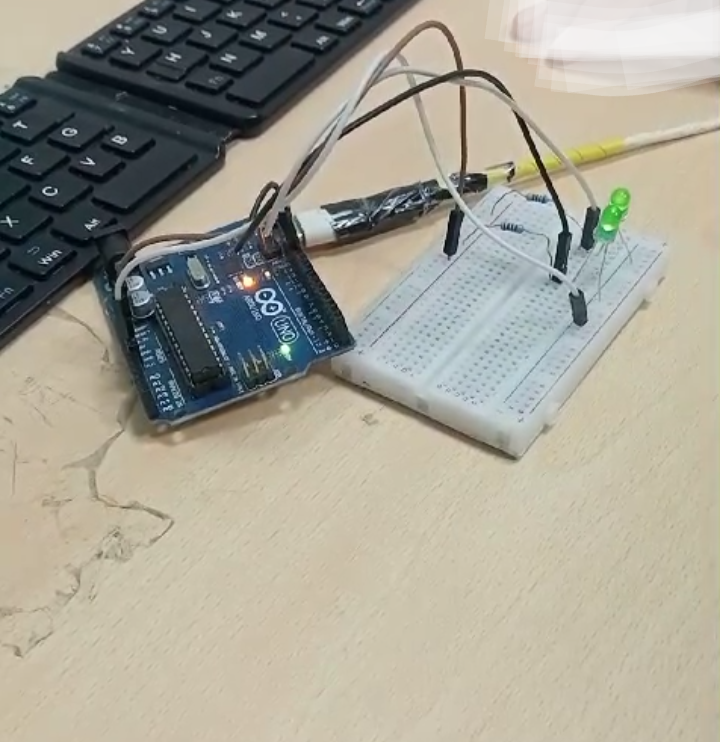
\includegraphics[width=0.4\textwidth]{fig.jpg}
   \caption{\label{fig:1}}
  \end{figure}

 \section{CONCLUSION}

The provided Arduino code successfully implements a JK flip-flop using software. The circuit utilizes two flip-flops, $Q1$ and $Q2$, to generate a specific sequence of outputs based on a clock input. 





\end{document}

